\textbf{\underline{\smash{Supercritical Pitchfork bifurcation}}}\vspace{0.2cm}\\
Normal form: $\dot{x}=rx-x^3$\\
Note that this equation is invariant under the exchange of the variable $x\to -x$. We get the following vector fileds for different values of $r$
\begin{figure}[H]
	\centering
	\begin{multicols}{2}
		\begin{figure}[H]
			\begin{tikzpicture}
				\draw[->] (-2,0)--(2,0)node[below right]{$x$};
				\draw[->] (0,-2)--(0,2)node[above left]{$\dot{x}$};
				\draw[domain={-2^(1/3)}:{2^(1/3)},samples=50] plot(\x,{-(\x)^3});
				\node[above right] at (-2,2){$r\leq 0$};
				\draw[fill=black] (0,0)circle(2pt);
			\end{tikzpicture}
		\end{figure}\columnbreak
		\begin{figure}[H]
			\begin{tikzpicture}
				\draw[->] (-2,0)--(2,0)node[below right]{$x$};
				\draw[->] (0,-2)--(0,2)node[above left]{$\dot{x}$};
				\draw[domain={-2^(1/3)-0.25}:{2^(1/3)+0.25},samples=50] plot(\x,{\x-(\x)^3});
				\node[above right] at (-2,2){$r>0$};
				\draw[fill=black] (-1,0)circle(2pt)(1,0)circle(2pt);
				\draw[fill=white] (0,0)circle(2pt);
			\end{tikzpicture}
		\end{figure}
	\end{multicols}
\end{figure}
\noindent At $r=0$ we observe a transition from a single stable Fixpoint at $x^\ast=\pm\sqrt{r}$. The fixpoint at $x^\ast=0$ gets unstable.\vspace{0.2cm}\\
\underline{\smash{Bifurcation diagram}}:
\begin{figure}[H]
	\centering
	\begin{tikzpicture}
		\draw (-3,0)--(0,0);
		\draw[->,dashed] (0,0)--(3,0)node[below right]{$r$};
		\draw[->] (0,-3)--(0,3)node[above left]{$x$};
		\draw[domain={-3^(0.5):3^(0.5)},samples=50] plot({(\x)^2},\x);
	\end{tikzpicture}
\end{figure}
\noindent \underline{\smash{Example}}: We consider the potential $V(x)$ for the system $\dot{x}=rx-x^3$.\\
The potential is given by $f(x)=-\frac{dV}{dx} \leadsto V(x)=-\frac{1}{2}rx^2+\frac{1}{4}x^4$
\begin{figure}[H]
	\centering
	\begin{multicols}{2}
		\begin{figure}[H]
			\begin{tikzpicture}
				\draw[->] (-2,0)--(2,0)node[below right]{$x$};
				\draw[->] (0,-2)--(0,2)node[above left]{$\dot{x}$};
				\draw[domain={-2^(1/4)}:{2^(1/4)},samples=50] plot(\x,{(\x)^4});
				\node[above right] at (-2,2){$r\leq 0$};
			\end{tikzpicture}
		\end{figure}\columnbreak
		\begin{figure}[H]
			\begin{tikzpicture}
				\draw[->] (-2,0)--(2,0)node[below right]{$x$};
				\draw[->] (0,-2)--(0,2)node[above left]{$\dot{x}$};
				\draw[domain={-2^(1/4)-0.75}:{2^(1/4)+0.75},samples=50] plot(\x,{-1/2*(\x)^2+((\x)^4)/4});
				\node[above right] at (-2,2){$r>0$};
			\end{tikzpicture}
		\end{figure}
	\end{multicols}
\end{figure}
\vspace{0.2cm}\noindent \textbf{\underline{\smash{Subcritical pitchfork bifurcation}}}\\
Normal form: $\dot{x}=rx+x^3 \leftarrow$ the cubix term is destabilizing.\vspace{0.2cm}\\
\underline{\smash{Bifurcation diagram}}
\begin{figure}[H]
	\centering
	\begin{multicols}{2}
		\begin{figure}[H]
			\begin{tikzpicture}
				\draw (-3,0)--(0,0);
				\draw[->,dashed] (0,0)--(3,0)node[below right]{$r$};
				\draw[->] (0,-3)--(0,3)node[above left]{$x$};
				\draw[dashed,domain={-3^(0.5):3^(0.5)},samples=50] plot({-(\x)^2},\x);
			\end{tikzpicture}
		\end{figure}\columnbreak
		The nonzero fixed points are located at $x^\ast=\pm\sqrt{r}$. The are unstable.
	\end{multicols}
\end{figure}
\noindent The pitchfork-bifurcation is inverted.\\
\textbf{Remark}: In real physical systems one often has a stabilizing higher order term, such that a canonical form of a system with a subcritical pitchfork bifurcation is given by: $\dot{x}=xr+x^3-x^5$. The system has still the $x\to -x$ symmetry.
\begin{figure}[H]
	\centering
	\begin{multicols}{2}
		\begin{figure}[H]
			\begin{tikzpicture}
				\draw (-3,0)--(0,0);
				\draw[->,dashed] (0,0)--(3,0)node[below right]{$r$};
				\draw[->] (0,-3)--(0,3)node[above left]{$x$};
				\draw[dashed,domain={-1^(0.5):1^(0.5)},samples=50] plot({-(\x)^2},\x);
				\draw[domain=1:{5^(1/4)},samples=50] plot({(\x)^4-2},\x);
				\draw[domain=-1:{-5^(1/4)},samples=50] plot({(\x)^4-2},\x);
				\draw (-1,0.1)--(-1,-0.1)node[below]{$r_s$};
				\draw[->,shorten <= 3pt, shorten >= 3pt] (-1,1)--(-1,0.1);
				\node[right] at (1,0.75){hysteresis};
			\end{tikzpicture}
		\end{figure}\columnbreak
		\textbf{Remark}:
		\begin{enumerate}[label={$\arabic*)$}]
			\item In the range $r_s<r<0$ two qualitatively different stable fixed points exist. The fixed points at the origin is \underline{\smash{locally}} stable, since for large values of $x_0$ the system may converge to the large amplitude fixed point.
			\item We may observe jumps and hysteresis upon variation of $r$.
			\item the bifurcation at $r_s$ is a saddle-node bifurcation.
		\end{enumerate}
	\end{multicols}
\end{figure}
\subsubsection{Flows on the circle}
We now consider vector fields as the following: $\dot{\theta}=f(\theta)$ where $\theta$ is a point on a circle and $\dot{\theta}$ is the velocity vector at that point. This choice of the variable allowsus to get periodic solutions in a 1D-system.\vspace{0.2cm}\\
\underline{Example}: Vector filed corresponding to $\dot{\theta}=\sin(\theta)$
\begin{figure}[H]
	\centering
	\begin{multicols}{2}
		\begin{figure}[H]
			\centering
			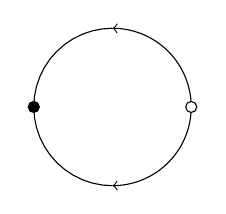
\begin{tikzpicture}
				\draw[domain=90:270,samples=25] plot({cos(\x)},{sin(\x)});
				\draw[->,domain=0:90,samples=25] plot({cos(\x)},{sin(\x)});
				\draw[->,domain=0:90,samples=25] plot({cos(\x)},{-sin(\x)});
				\draw[fill=white] (1,0)circle(2pt);
				\draw[fill=black] (-1,0)circle(2pt);
			\end{tikzpicture}
		\end{figure}\columnbreak
		\begin{figure}[H]
			\centering
			\begin{tikzpicture}
				\draw[->] (-2.5,0)--(2.5,0)node[below right]{$\theta$};
				\draw[->] (0,-1.5)--(0,1.5)node[above left]{$\dot{\theta}$};
				\draw[domain=-2.5:2.5,samples=100] plot(\x,{sin(90*\x)});
				\draw[fill=black] (-2,0)circle(2pt)(2,0)circle(2pt);
				\draw[fill=white] (0,0)circle(2pt);	
			\end{tikzpicture}
		\end{figure}
	\end{multicols}
\end{figure}
\noindent A vector field on a circle is a rule that assigns a unique velocity vector to a point on the circle. Therefore $f(\theta)$ has to be a periodic function. There is for example no unique velocity for $\dot{\theta}=\theta$ since $\theta=0$ and $\theta=2\pi$ correspond to the same point on a circle but to different velocities.\vspace{0.5cm}\\
\textbf{\underline{\smash{Uniform oscillator}}}: A point on a circle is often called phase or angle. And the simplest oscillator is given by $\dot{\theta}=\omega\leadsto\theta(t)=\omega t+\theta_0$. After the period of $T=\frac{2\pi}{\omega}$ the oscillator returns to the same point.\vspace{0.5cm}\\
\textbf{\underline{\smash{Nonuniform oscillator}}}: $\dot{\theta}=\omega-a\sin(\theta)\quad ,a,\omega>0$\vspace{0.2cm}\\
In this realization of the oscillator its velocity is not constant anymore.
\begin{figure}[H]
	\centering
	\begin{tikzpicture}
		\draw[->] (-3,0)--(3,0)node[below right]{$\theta$};
		\draw[->] (0,-3)--(0,3)node[above left]{$\dot{\theta}$};
		\draw[domain=-3:3,samples=50] plot(\x,{-sin(90*\x)+1.2});
		\draw (-0.1,1.2)--(0.1,1.2)node[right]{$\omega$};
		\draw[dashed] (1,0.2)--(1,1.2)node[midway,right]{$a$};
	\end{tikzpicture}
\end{figure}
We now discuss the parameter space of the system:
\begin{itemize}
	\item[$a=0$] We return to the uniform oscillator
	\item[$a\neq 0$] $\theta=-\frac{\pi}{2}$ corresponds to the fastest flow, $\theta=\frac{pi}{2}$ the slowest flow
\end{itemize}
\underline{Bottleneck}: If $\omega>0$ but $\omega -a<<1$ the system slows down considerably. The phase point $\theta(t)$ takes a long time to passt the bottleneck. For $a\geq\omega$ the oscillator stops.
\begin{figure}[H]
	\centering
	\begin{multicols}{2}
		\begin{figure}[H]
			\centering
			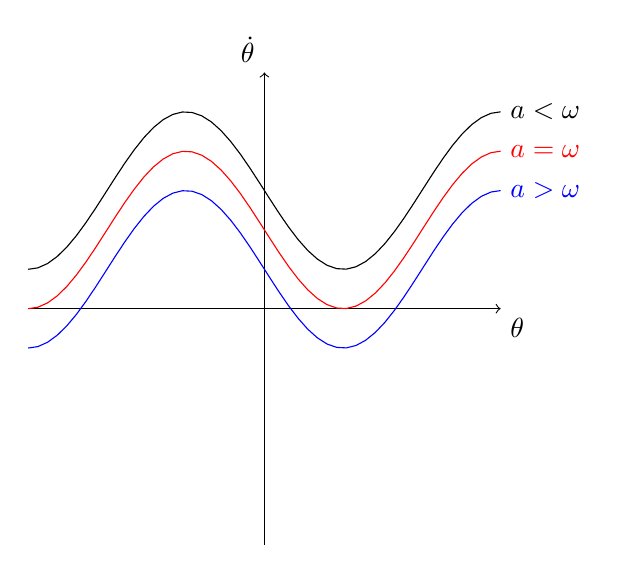
\begin{tikzpicture}
				\draw[->] (-3,0)--(3,0)node[below right]{$\theta$};
				\draw[->] (0,-3)--(0,3)node[above left]{$\dot{\theta}$};
				\draw[domain=-3:3,samples=50] plot(\x,{-sin(90*\x)+1.5});
				\node[right] at (3,2.5){$a<\omega$};
				\draw[red,domain=-3:3,samples=50] plot(\x,{-sin(90*\x)+1});
				\node[red,right] at (3,2){$a=\omega$};
				\draw[blue,domain=-3:3,samples=50] plot(\x,{-sin(90*\x)+0.5});
				\node[blue,right] at (3,1.5){$a>\omega$};
			\end{tikzpicture}
		\end{figure}\columnbreak
		\begin{figure}[H]
			\begin{multicols}{2}
				\begin{figure}[H]
					\centering
					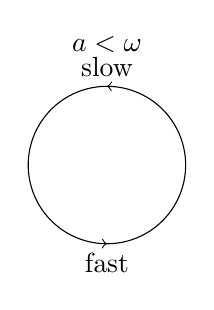
\begin{tikzpicture}
						\draw[->,domain=-90:90,samples=50] plot({cos(\x)},{sin(\x)})node[above]{slow};
						\draw[->,domain=90:270,samples=50] plot({cos(\x)},{sin(\x)})node[below]{fast};
						\node[above] at (0,1.3){$a<\omega$};
					\end{tikzpicture}
				\end{figure}\columnbreak
				\begin{figure}[H]
					\centering
					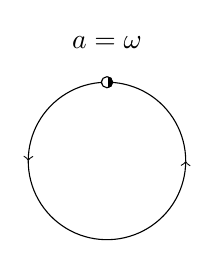
\begin{tikzpicture}
						\draw[->,domain=0:180,samples=50] plot({cos(\x)},{sin(\x)});
						\draw[->,domain=180:360,samples=50] plot({cos(\x)},{sin(\x)});
						\draw[fill=black] (0,1)circle(2pt);
						\draw[white,fill=white] (-0.05,0.9)--(-0.05,1.1)--(0,1.1)--(0,0.9)--cycle;
						\draw (0,1)circle(2pt);
						\node[above] at (0,1.3){$a=\omega$};
					\end{tikzpicture}
				\end{figure}
			\end{multicols}
			\begin{figure}[H]
				\centering
				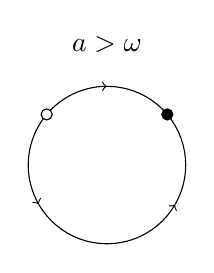
\begin{tikzpicture}
					\draw[->,domain=120:90] plot({cos(\x)},{sin(\x)});
					\draw[->,domain=120:210] plot({cos(\x)},{sin(\x)});
					\draw[->,domain=210:330] plot({cos(\x)},{sin(\x)});
					\draw[domain=330:450] plot({cos(\x)},{sin(\x)});
					\node[above] at (0,1.3){$a>\omega$};
					\draw[fill=white] ({cos(140)},{sin(140)})circle(2pt);
					\draw[fill=black] ({cos(40)},{sin(40)})circle(2pt);
				\end{tikzpicture}
			\end{figure}
		\end{figure}
	\end{multicols}
\end{figure}
For this simple system one can calculate the oscillation period as well
\begin{equation*}
	T=\int dt=\int\limits_0^{2\pi} \frac{dt}{d\theta}d\theta=\int\limits_0^{2\pi}\frac{d\theta}{\omega-a\sin(\theta)}=\frac{2\pi}{\sqrt{\omega^2-a^2}}
\end{equation*}
\begin{figure}[H]
	\centering
	\begin{multicols}{2}
		\begin{figure}[H]
			\centering
			\begin{tikzpicture}
				\draw[->] (-0.5,0)--(3,0)node[below right]{$a$};
				\draw[->] (0,-0.5)--(0,3)node[above left]{$T(a)$};
				\draw (0.1,1/3)--(-0.1,1/3)node[left]{$\frac{2\pi}{\omega}$};
				\draw[domain=0:2.98,samples=50] plot(\x,{1/sqrt(3^2-(\x)^2)});
			\end{tikzpicture}
		\end{figure}\columnbreak
		Obviously, we get $T=\frac{2\pi}{\omega}$ for $a=0$. The order of the divergence can be obtained from
		\begin{equation*}
			\sqrt{\omega^2-a^2}=\sqrt{\omega+a}\sqrt{\omega-a}\underset{\omega\approx a}{=}\sqrt{2\omega}\sqrt{\omega-a}
		\end{equation*}
		\begin{equation*}
			T\approx\frac{\pi\sqrt{2}}{\sqrt{\omega}}\frac{1}{\sqrt{\omega-a}}\approx (a_c-a)^{-\frac{1}{2}}
		\end{equation*}
	\end{multicols}
\end{figure}
This behaviour is generic, since it is driven by the local minimum of $\dot{\theta}$ at $a=a_c$. Therefore the bottleneck can be described by:
\begin{equation*}
	\dot{x}=r+x^2\qquad (0<r<<1)
\end{equation*}
\begin{equation*}
	T_\text{bottleneck}\approx\int\limits_{-\infty}^\infty\frac{dx}{r+x^2}=\frac{\pi}{\sqrt{r}}
\end{equation*}
i.e. the square root scaling law
\begin{figure}[H]
	\centering
	\begin{tikzpicture}
		\draw[->] (-2,0)--(2,0)node[below right]{$x$};
		\draw[->] (0,-2)--(0,2)node[above left]{$\dot{x}$};
		\draw[domain={-sqrt(2)}:{sqrt(2)},samples=50] plot(\x,{0.1+(\x)^2});
	\end{tikzpicture}
\end{figure}
